\section{Nuevas Áreas de Aplicación de la IA en la Industria Farmacéutica}

\subsection{Introducción}

La Inteligencia Artificial (IA) está revolucionando la industria farmacéutica, especialmente en la gestión de materias primas y el control de procesos. Más allá de los enfoques tradicionales como los sistemas de gestión de inventarios, la IA ofrece oportunidades innovadoras en áreas como el control de temperatura y el análisis de datos no supervisado. Estas tecnologías no solo permiten la optimización de recursos, sino que también mejoran la calidad y la seguridad de los productos farmacéuticos.

\subsection{Aplicaciones del Aprendizaje No Supervisado en la Industria Farmacéutica}

El aprendizaje no supervisado es una rama de la IA que se enfoca en encontrar patrones en datos sin la necesidad de etiquetas o supervisión humana. En la industria farmacéutica, el aprendizaje no supervisado puede aplicarse para detectar anomalías en la calidad de las materias primas, optimizar el control de procesos y analizar grandes volúmenes de datos.

\subsubsection{1. Detección de Anomalías en Materias Primas}

El control de calidad de las materias primas es un desafío constante en la industria farmacéutica. Con algoritmos de clustering no supervisados, como \textit{k-means} o redes neuronales autoorganizadas (SOM), es posible identificar patrones anómalos en los lotes de materias primas que podrían pasar desapercibidos con técnicas tradicionales.

\textbf{Beneficios}:
\begin{itemize}
    \item Mejora en la detección temprana de defectos o contaminación.
    \item Reducción de riesgos en la cadena de producción.
    \item Optimización del control de calidad mediante análisis automatizados.
\end{itemize}

\textbf{Tecnologías Clave}:
\begin{itemize}
    \item \textit{k-means clustering}: Agrupa las muestras en base a similitudes, permitiendo identificar grupos anómalos.
    \item \textit{Autoencoders}: Redes neuronales que identifican patrones no típicos basándose en la compresión de datos.
    \item \textit{Análisis de Componentes Principales (PCA)}: Permite reducir la dimensionalidad de los datos para detectar outliers.
\end{itemize}

\subsubsection{2. Optimización del Proceso de Fabricación}

El aprendizaje no supervisado también puede optimizar los procesos de fabricación farmacéutica mediante el análisis de datos de sensores y máquinas que controlan variables clave, como la temperatura, la presión o la humedad. La IA puede identificar combinaciones óptimas de variables para mejorar la eficiencia y reducir el consumo de energía.

\textbf{Beneficios}:
\begin{itemize}
    \item Aumento de la eficiencia de la producción.
    \item Reducción de costos energéticos.
    \item Mejora en la consistencia y calidad del producto final.
\end{itemize}

\textbf{Tecnologías Clave}:
\begin{itemize}
    \item \textit{Mapas Autoorganizados (SOM)}: Utilizados para monitorear y ajustar los parámetros de fabricación en tiempo real.
    \item \textit{Algoritmos de clustering jerárquico}: Para descubrir correlaciones entre las variables de control de proceso.
\end{itemize}

\subsection{Control de Temperatura Inteligente con IA}

El control preciso de la temperatura es esencial en la industria farmacéutica, especialmente en la fabricación y almacenamiento de medicamentos sensibles. La IA, en combinación con sistemas de monitoreo de temperatura, puede proporcionar ajustes automáticos en tiempo real, asegurando que los productos se mantengan en un rango óptimo.

\subsubsection{1. Monitoreo Predictivo de Temperatura}

Utilizando algoritmos de predicción basados en IA, es posible anticipar cambios en la temperatura dentro de los sistemas de almacenamiento o durante el transporte, lo que permite realizar ajustes antes de que los parámetros se desvíen fuera de los rangos aceptables.

\textbf{Beneficios}:
\begin{itemize}
    \item Reducción de pérdidas de productos por condiciones inadecuadas de temperatura.
    \item Mejora en la trazabilidad y seguridad del producto.
    \item Respuesta más rápida ante anomalías en las condiciones de almacenamiento.
\end{itemize}

\textbf{Tecnologías Clave}:
\begin{itemize}
    \item \textit{Redes Neuronales Recurrentes (RNN)}: Para predecir fluctuaciones de temperatura basadas en datos históricos.
    \item \textit{Modelos de Predicción Basados en Series Temporales}: Para identificar patrones de comportamiento térmico y prevenir desviaciones.
\end{itemize}

\subsubsection{2. Gestión de Almacenes Inteligentes Basada en Temperatura}

La IA también puede mejorar la disposición de productos farmacéuticos en almacenes, ubicándolos estratégicamente según sus necesidades específicas de temperatura. Esto es particularmente útil para productos que deben mantenerse en condiciones de frío o ambientes controlados.

\textbf{Beneficios}:
\begin{itemize}
    \item Optimización del uso de energía en sistemas de refrigeración.
    \item Mejora en la seguridad del almacenamiento de productos termolábiles.
    \item Reducción de desperdicios por caducidad temprana o deterioro por exposición térmica.
\end{itemize}

\textbf{Tecnologías Clave}:
\begin{itemize}
    \item \textit{Sensores IoT Integrados con IA}: Para monitorear en tiempo real la distribución de temperatura en los almacenes.
    \item \textit{Algoritmos de Optimización}: Para mejorar la disposición física de los productos y minimizar la variabilidad térmica.
\end{itemize}

\subsection{Análisis de Datos No Supervisado para la Seguridad de Medicamentos}

La IA no supervisada también puede ayudar en la farmacovigilancia, detectando patrones inusuales en los reportes de efectos adversos. El análisis de grandes volúmenes de datos sobre reacciones adversas puede identificar grupos de riesgo o correlaciones no evidentes entre los efectos secundarios y ciertos tipos de medicamentos o pacientes.

\textbf{Beneficios}:
\begin{itemize}
    \item Detección más rápida de riesgos para la seguridad de medicamentos.
    \item Reducción de riesgos asociados a reacciones adversas graves.
    \item Mejora en la toma de decisiones para la regulación y autorización de fármacos.
\end{itemize}

\textbf{Tecnologías Clave}:
\begin{itemize}
    \item \textit{Algoritmos de Clustering}: Para agrupar reportes similares de efectos adversos.
    \item \textit{Modelos de Análisis de Redes}: Para identificar relaciones entre los medicamentos y los grupos de pacientes.
\end{itemize}

\subsection{Conclusión}

El uso de IA, especialmente el aprendizaje no supervisado, ofrece un gran potencial para optimizar la gestión de materias primas y el control de procesos en la industria farmacéutica. Desde el monitoreo predictivo de la temperatura hasta la detección de anomalías en las materias primas, estas tecnologías permiten una mejora significativa en la eficiencia, calidad y seguridad del sector, manteniendo siempre la precisión que exige la industria.

\section{Comparación de Resultados: Antes y Después de la Implementación de IA}

\subsection{Control de Calidad de Materias Primas}

El siguiente cuadro muestra la diferencia en el control de calidad de materias primas antes y después de implementar técnicas de IA no supervisadas para la detección de anomalías.

\begin{table}[H]
\centering
\caption{Comparación de Control de Calidad de Materias Primas (Antes y Después de IA)}
\resizebox{\textwidth}{!}{
\begin{tabular}{@{}lcc@{}}
\toprule
\textbf{Aspecto} & \textbf{Antes de Implementar IA} & \textbf{Después de Implementar IA} \\ \midrule
Tasa de detección de defectos & Baja, basada en inspección manual & Alta, con detección automatizada por IA \\
Tiempo de detección de anomalías & Lento, inspección manual lote por lote & Rápido, análisis en tiempo real con clustering \\
Consistencia en la calidad & Variable debido a errores humanos & Alta consistencia gracias a IA automatizada \\
Costos de inspección & Altos debido al trabajo manual intensivo & Reducción significativa de costos \\ \bottomrule
\end{tabular}}
\end{table}

\subsection{Control de Temperatura en Almacenamiento}

La siguiente tabla compara el control de temperatura en almacenes farmacéuticos antes y después de la implementación de IA para el monitoreo y ajuste predictivo.

\begin{table}[H]
\centering
\caption{Comparación del Control de Temperatura (Antes y Después de IA)}
\resizebox{\textwidth}{!}{
\begin{tabular}{@{}lcc@{}}
\toprule
\textbf{Aspecto} & \textbf{Antes de Implementar IA} & \textbf{Después de Implementar IA} \\ \midrule
Monitoreo de temperatura & Manual o reactivo ante problemas & Predicción y ajuste en tiempo real con IA \\
Tiempo de respuesta ante desviaciones & Lento, con posibles daños a los productos & Inmediato, previniendo riesgos de deterioro \\
Costos de energía & Altos por ineficiencia en la refrigeración & Reducción de costos por optimización energética \\
Pérdida de productos & Alta por fallas en el control de temperatura & Significativamente reducida gracias al monitoreo predictivo \\ \bottomrule
\end{tabular}}
\end{table}

\subsection{Diagrama: Proceso de Implementación de IA en Control de Materias Primas y Temperatura}

A continuación se presenta un diagrama de flujo que describe el proceso de implementación de IA en la detección de anomalías en materias primas y en el control de temperatura en almacenes.

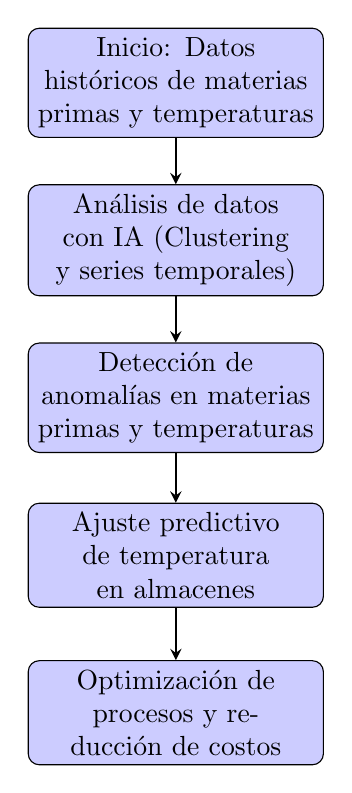
\begin{tikzpicture}[node distance=2cm, auto]
% Styles
\tikzstyle{block} = [rectangle, draw, fill=blue!20, text centered, rounded corners, minimum height=2em, text width=10em]
\tikzstyle{arrow} = [thick,->,>=stealth]

% Nodes
\node (start) [block] {Inicio: Datos históricos de materias primas y temperaturas};
\node (analyze) [block, below of=start] {Análisis de datos con IA (Clustering y series temporales)};
\node (detect) [block, below of=analyze] {Detección de anomalías en materias primas y temperaturas};
\node (adjust) [block, below of=detect] {Ajuste predictivo de temperatura en almacenes};
\node (optimize) [block, below of=adjust] {Optimización de procesos y reducción de costos};

% Arrows
\draw [arrow] (start) -- (analyze);
\draw [arrow] (analyze) -- (detect);
\draw [arrow] (detect) -- (adjust);
\draw [arrow] (adjust) -- (optimize);
\end{tikzpicture}
